
\appendix*

\section{}

\begin{figure*}[h!]
	\subfigure[]{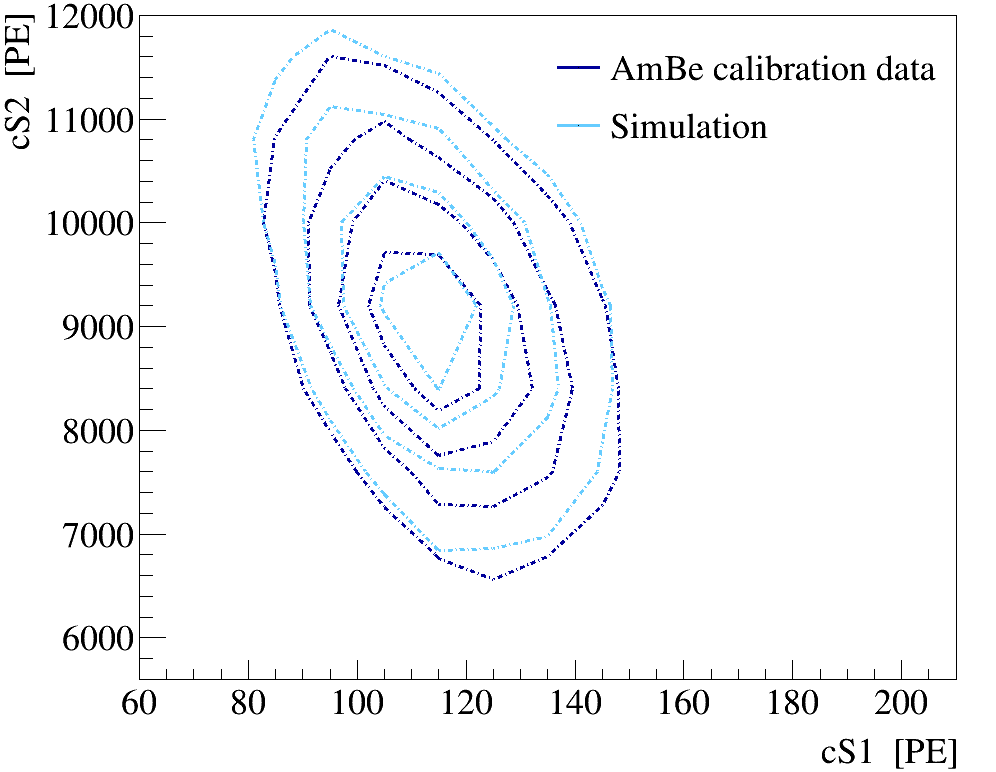
\includegraphics[width=0.49\linewidth]{images/mc_ambe_comp_contour.png}}
	\subfigure[]{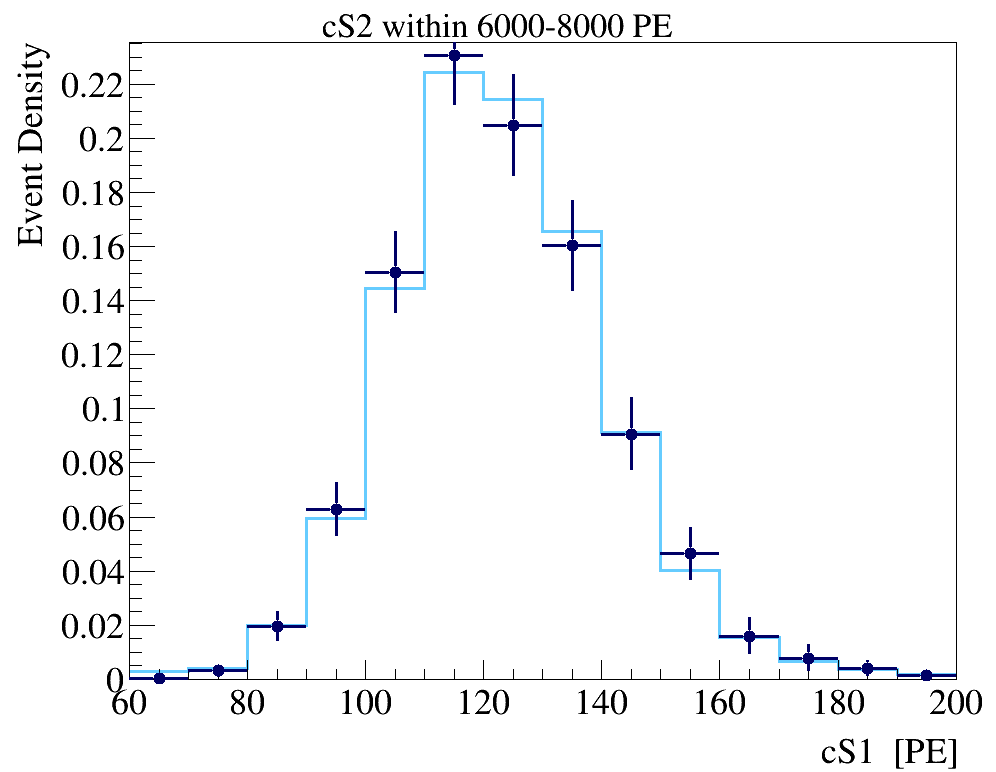
\includegraphics[width=0.49\linewidth]{images/mc_ambe_comp_slice1.png}} \\
	\subfigure[]{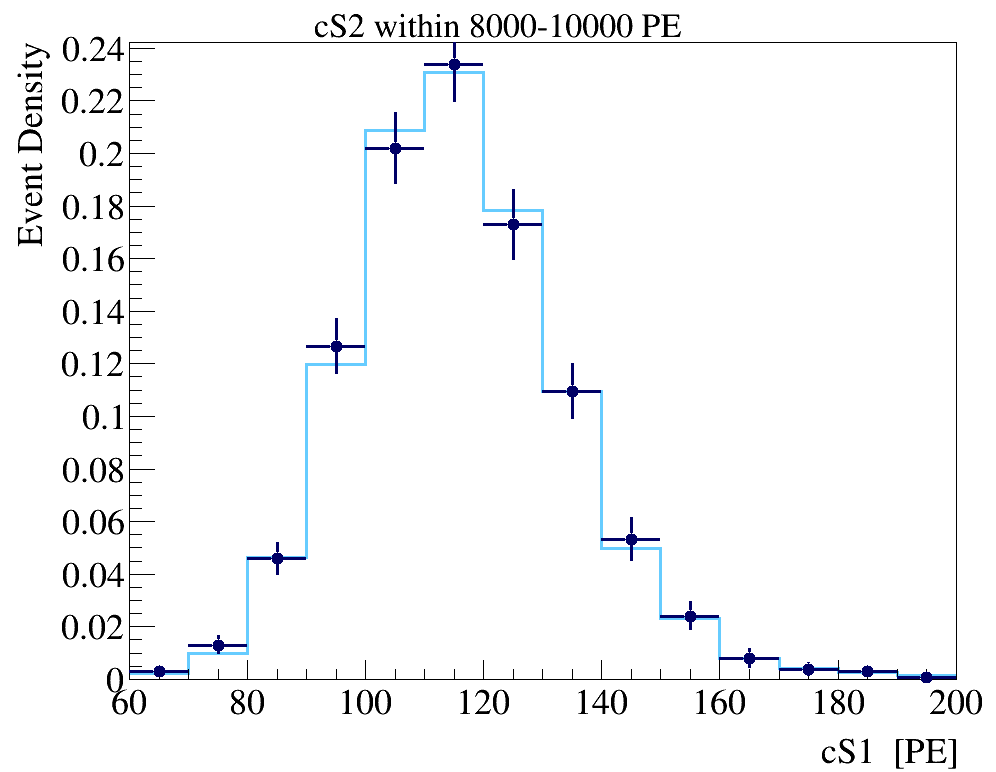
\includegraphics[width=0.49\linewidth]{images/mc_ambe_comp_slice2.png}}
	\subfigure[]{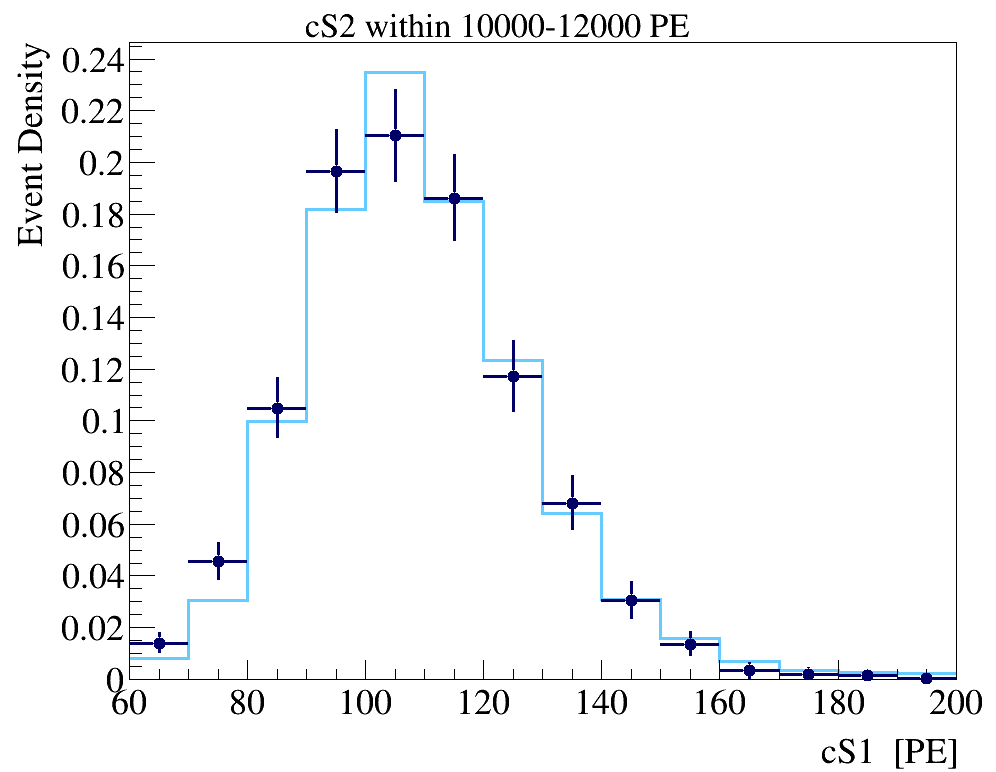
\includegraphics[width=0.49\linewidth]{images/mc_ambe_comp_slice3.png}}
	\caption{A simulation of the 39.6\,keV  xenon line activated from $^{243}$AmBe neutrons is compared with the actual data.
		 Figure~(a) compare contours of equal density in the (cS1,cS2)-plane, while Figures~(b), (c) and (d) shows the same distribution projected in cS1 for
		 several ranges of cS2, the histograms are normalized to unit area. Light and dark blue represent simulation and data, respectively.
		}
		
  \label{fig:mc_comp}
\end{figure*}

The detector response to inelastic WIMP-$^{129}$Xe interactions was simulated using an empirical signal model. 
The procedure, described in detail in section~\ref{sec:signal}, take advantage of several 
assumptions and approximations which have been validated extensively. 
The main cross check was to reproduce with simulation the 39.6\,keV xenon line activated from $^{124}$AmBe neutrons. 
For this purpose the NR energy spectrum expected from inelastic neutron-$^{129}$Xe scattering has been obtained via  Monte Carlo techniques, 
we take into account detector response and the non-uniform spatial distribution. Acceptance of analysis selections to this type of interaction 
have been recomputed accordingly, in particular, acceptance to the double scatter cut differ greatly between neutrons and WIMPs scattering. 
Except for acceptances and NR energy spectrum the simulation has been performed following the receipt described in the main text. Figure~\ref{fig:mc_comp}
shows a comparisons between simulation (light blue) and calibration data (dark blue), contour lines of equal densities are compared in Figure~(a), 
while Figures~(b), (c) and (d) shows cS1 projected distributions for different ranges in cS2.


